\subsection{Results: Grid search on CNN}

\subsubsection{Number of Linear Layers and Nodes}



\begin{figure}[H]
    \centering
    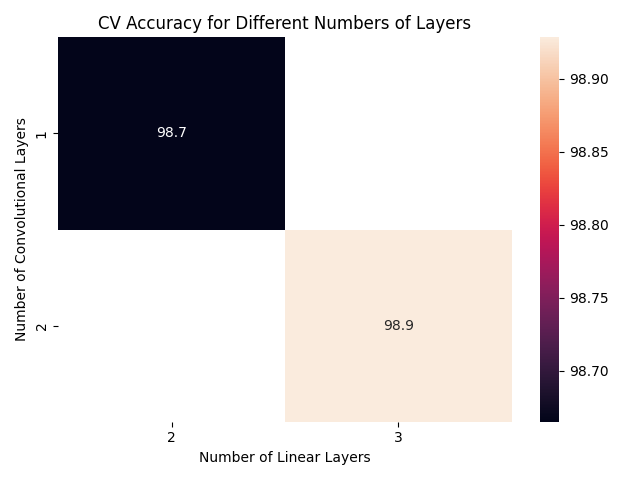
\includegraphics[width=\textwidth]{results/cnn_grid_search/heatmap_grid_search_layers.png}
    \caption{CNN gridsearch for 3 different values of kernel size and filter size. Learning rate is 0.001.}
    \label{fig:LogRegEpochs}
\end{figure}

\newpage
As we can see from Figure \ref{fig:LogRegLearningRate}, the model accuracy increases from the smallest learning rate up until the largest learning rate. The biggest accuracy achieved is about 91\%.

\begin{figure}[H]
    \centering
    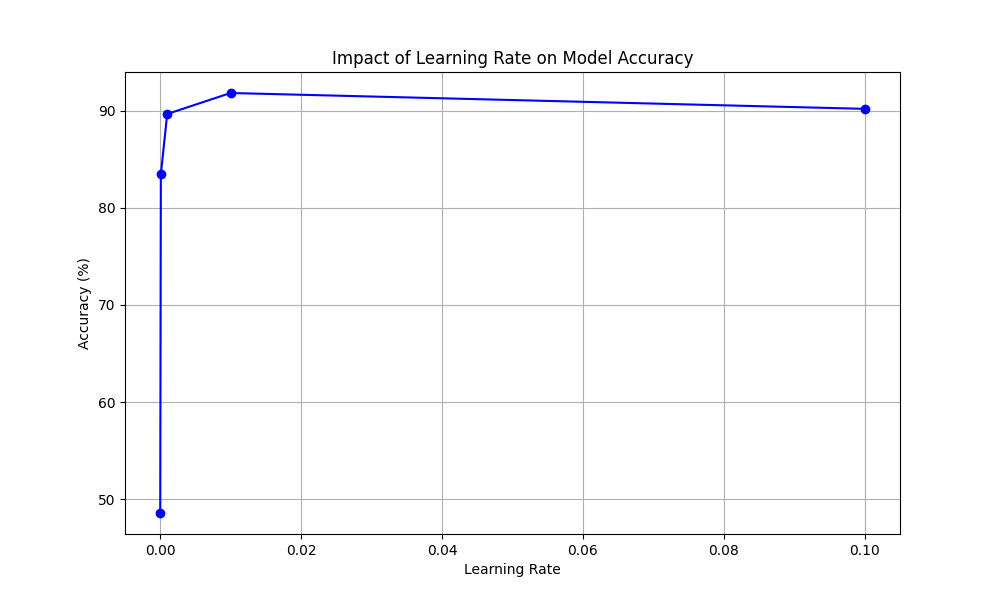
\includegraphics[width=\textwidth]{results/logreg/learning_rate_study.png}
    \caption{Logistic regression classification with learningrates in the range from $10^{-5}$ to $10^0$.}
    \label{fig:LogRegLearningRate}
\end{figure}

From Figure \ref{fig:LogRegEpochs} we can see that number of epochs does not have any effect on accuracy. An accuracy of about 89\% was achieved with all number of epochs. It was considered to run more epochs but because of the diminishing returns when epochs increases we decided to save computational resources. 

\begin{figure}[H]
    \centering
    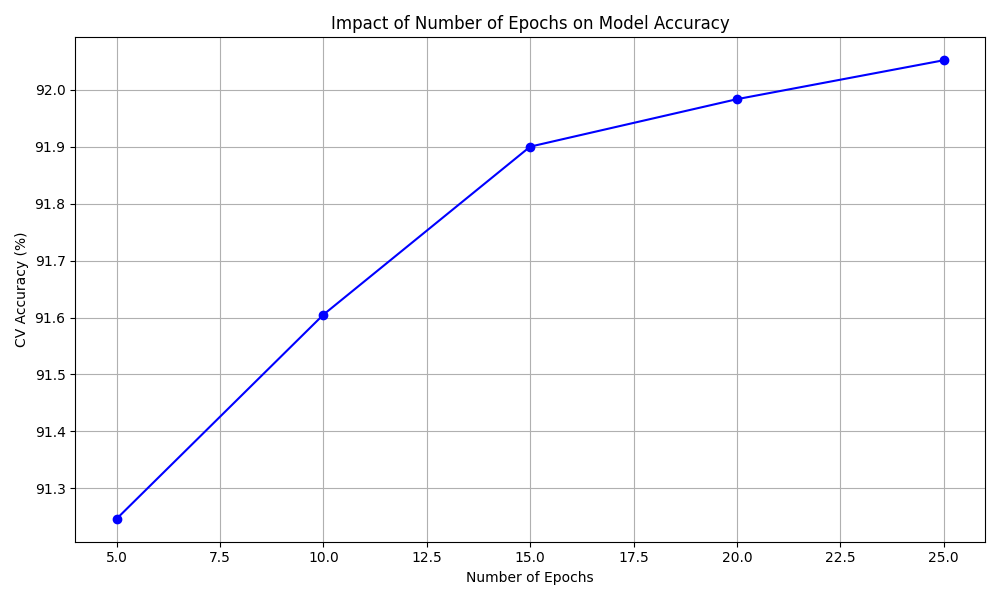
\includegraphics[width=\textwidth]{results/logreg/number_of_epochs_study.png}
    \caption{Logistic regression classification with epochs in the range from $5$ to $25$.}
    \label{fig:LogRegEpochs}
\end{figure}

Moving on to Figure \ref{fig:LogRegBatchsize} we can see that in contrast to number of epochs, the increasing of batch size lowers accuracy. The biggest accuracy was around 91\% when a batch size of 15 was used. It should be noted that the absolute value decrease of around 4\% for batch size and 0\% for epochs is not that big. This indicates that these two variables are less important in optimizing for accuracy than learning rate which had a 70\% difference from lowest to biggest. 

\begin{figure}[H]
    \centering
    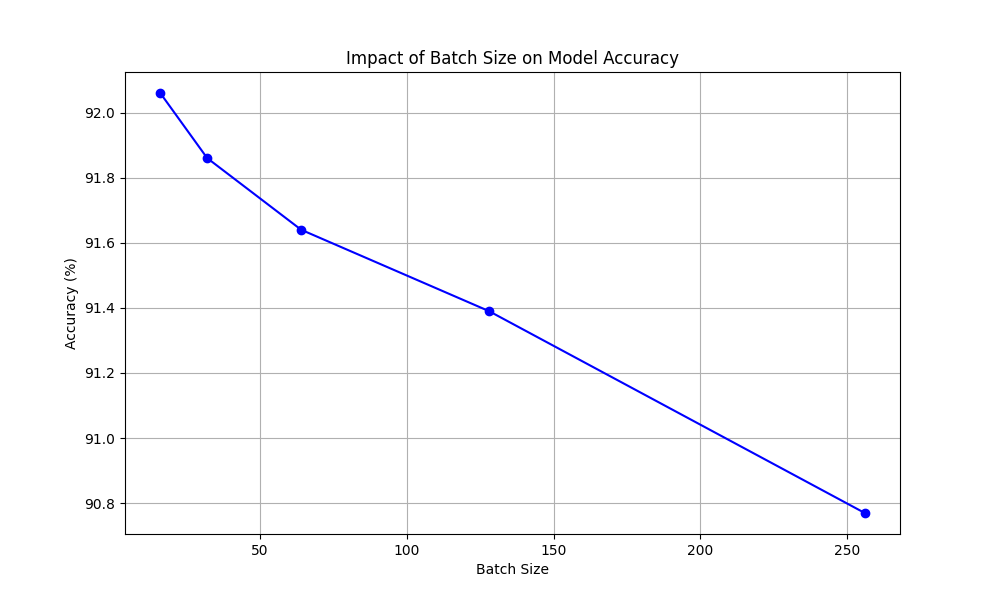
\includegraphics[width=\textwidth]{results/logreg/batch_size_study.png}
    \caption{Logistic regression classification with batchsize in the range from $16$ to $256$.}
    \label{fig:LogRegBatchsize}
\end{figure}

\subsection{Discussion of Performance}
The baseline vs CNN both reaches 90 \% without an extensive tuning of the baseline, which calls for the question if using convolutional neural networks are worth the trouble of runtime and reduced interpretability. However, in some applications of a model trained on the MNIST data set, such
as reading bank account numbers from handwritten digits, even tiny mistakes can be very costly.
Therefore, it is crucial to reduce this error as much as possible. \cite{raschka2022machine}

\iris {It should be noted that from the objective of performance, our tuning of hyperparameters could benefit from testing activation functions.}

A discussion: our results are highly sensitive to the initial values of our tuning. In a neural network, everything is interconnected, making it difficult to isolate individual effects. Earlier in this course, we spent considerable time examining how factors such as different learning rates, optimizers, and epochs influence learning convergence and model performance. In this project, however, we aimed to explore new hyper parameters specific to convolutional neural networks (CNNs): filter numbers, kernel size, dropout, padding, and pooling. Our focus on these new hyperparameters meant that we paid less attention to tuning the basic ones, which may have impacted our ability to achieve optimal model performance. For future work, we would like to explore more efficient methods of tuning neural networks, such as Bayesian optimization.

It was not fun to make a choice on the initial values, but we were forced to do it due to runtime. In the end we landed on making a choice we could argue, but in the perfect world we would test everything against each other. For computational resources, one could say that we chose a proper validation of the hyper parameters with cross-validation to take into account the randomness in different splits and model training, over testing everything against each other. 